\documentclass[a4paper,11pt]{article}

\usepackage[utf8]{inputenc}
\usepackage[T1]{fontenc}
\usepackage{lmodern}
\usepackage{amsmath}
\usepackage{graphicx}
\usepackage{booktabs}
\usepackage{hyperref}
\usepackage[margin=1cm]{geometry}
\usepackage{tikz}
\usetikzlibrary{positioning, arrows.meta, calc}

\definecolor{stefan}{RGB}{46,139,87}
\definecolor{chris}{RGB}{230,126,34}
\definecolor{christa}{RGB}{142,68,173}
\tikzset{
    comp/.style={draw, thick, rounded corners, minimum width=2.6cm, minimum height=0.9cm, align=center, font=\small},
    stefan/.style={comp, draw=stefan, fill=stefan!15},
    chris/.style={comp, draw=chris, fill=chris!15},
    christa/.style={comp, draw=christa, fill=christa!15},
    % shared component: left half Chris, right half Christa (fill and border)
    both/.style={comp, draw=none, path picture={
        \foreach \c/\a/\b in {chris/south west/south, christa/south/south east}{
            \begin{scope}
                \clip[sharp corners] (path picture bounding box.\a) rectangle (path picture bounding box.north -| path picture bounding box.\b);
                \fill[\c!15] (path picture bounding box.south west) rectangle (path picture bounding box.north east);
                \draw[\c, line width=1.6pt, rounded corners] (path picture bounding box.south west) rectangle (path picture bounding box.north east);
            \end{scope}
        }
    }},
    milestone/.style={draw, thick, fill=gray!10, minimum height=0.9cm, align=center, font=\small, text width=3.3cm},
    flow/.style={-{Stealth[length=2.5mm]}, thick},
    lbl/.style={font=\scriptsize, midway, fill=white, inner sep=1pt},
}

\title{BlueWasher protocol optimization with Chris(ta)}
\author{}
\date{}

\begin{document}

\maketitle
\section{Goal}
    We want to find a bluewasher protocol (or multiple) to wash plates up to twelve times with minimal loss of coverage of the well bottoms by cells.
    Maybe also an oracle telling how much coverage will be left after $n$ washed with protocol $P$.

\section{Final setup}
% tikz graph
% colors for components by person. stefan->green, chris->orange, christa purple
%nodes Agents, context, Interface service, Lab, WellEmpty-Check, CoverageCheck, Plates&Buffer, result database
\begin{figure}[h]
\centering
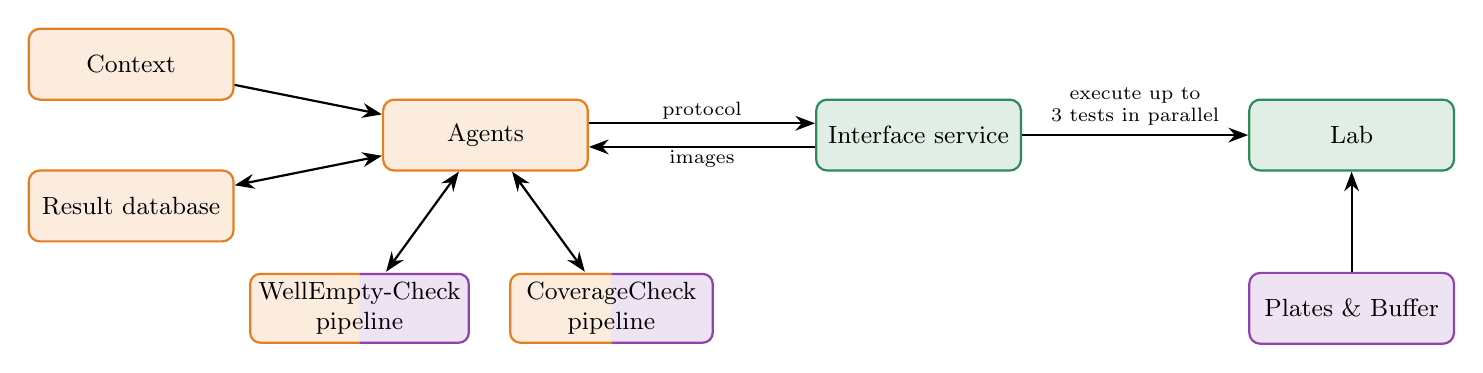
\begin{tikzpicture}
    \node[chris]   (context)   at (0,0.9)    {Context};
    \node[chris]   (db)        at (0,-0.9)   {Result database};
    \node[chris]   (agents)    at (4.5,0)    {Agents};
    \node[stefan]  (interface) at (10,0)     {Interface service};
    \node[stefan]  (lab)       at (15.5,0)   {Lab};
    \node[christa] (plates)    at (15.5,-2.2) {Plates \& Buffer};
    \node[both]    (empty)     at (2.9,-2.2) {WellEmpty-Check\\pipeline};
    \node[both]    (coverage)  at (6.1,-2.2) {CoverageCheck\\pipeline};

    \draw[flow] (context) -- (agents);
    \draw[flow, {Stealth[length=2.5mm]}-{Stealth[length=2.5mm]}] (db) -- (agents);
    \draw[flow] ([yshift=0.15cm]agents.east)    -- node[lbl, above]{protocol} ([yshift=0.15cm]interface.west);
    \draw[flow] ([yshift=-0.15cm]interface.west) -- node[lbl, below]{images}   ([yshift=-0.15cm]agents.east);
    \draw[flow] (interface) -- node[lbl, above=2pt, align=center]{execute up to\\3 tests in parallel} (lab);
    \draw[flow] (plates) -- (lab);
    \draw[flow, {Stealth[length=2.5mm]}-{Stealth[length=2.5mm]}] (agents) -- (empty);
    \draw[flow, {Stealth[length=2.5mm]}-{Stealth[length=2.5mm]}] (agents) -- (coverage);
\end{tikzpicture}

\vspace{0.5em}
\small
\tikz\node[stefan, minimum width=1cm, minimum height=0.4cm]{}; Stefan \quad
\tikz\node[chris, minimum width=1cm, minimum height=0.4cm]{}; Chris \quad
\tikz\node[christa, minimum width=1cm, minimum height=0.4cm]{}; Christa
\label{fig:setup}
\end{figure}
\subsection{Parts in detail:}
\paragraph{Context}
    A collection of example protocols, the BlueWasher manual and information on cell handling on the internet
\paragraph{Result database}
    Simple documentation of tests and their results including images. Should allow stop and resume of the whole optimization process
\paragraph{Interface service}
    A permanently running Python service (HTTP/JSON API, FastAPI) accepting certain functions:
    \begin{itemize}
        \item Accepts calls of type \texttt{test(protocol, n\_washes, coverage\_checks)} and returns a run-id
            \begin{itemize}
                \item \texttt{coverage\_checks}: list of the wash numbers after which the remaining coverage is checked(will be done after last in any case).
            \end{itemize}
        \item Provides the number of test calls that are currently accepted, i.e. if there is capacity left for more test runs on the platform
        \item Provides the status Waiting/Running/Finished/Failed of the test belonging to a run-id
        \item Provides the result, i.e. image-link to a run-id of a finished test
    \end{itemize}
\paragraph{Evaluation Pipelines}
    Callable functions doing the check.
\paragraph{Agents}
    Up to Chris. Since they never get called they do not need to implement any interface.


\section{Components and milestones}

\subsection{Road map}
%top->down graph showing order of milesstones and component completion
%components: interface service, coverage analysis pipeline, well empty check, loss function, protocol generation agent, optimization agent
\begin{figure}[h]
\centering
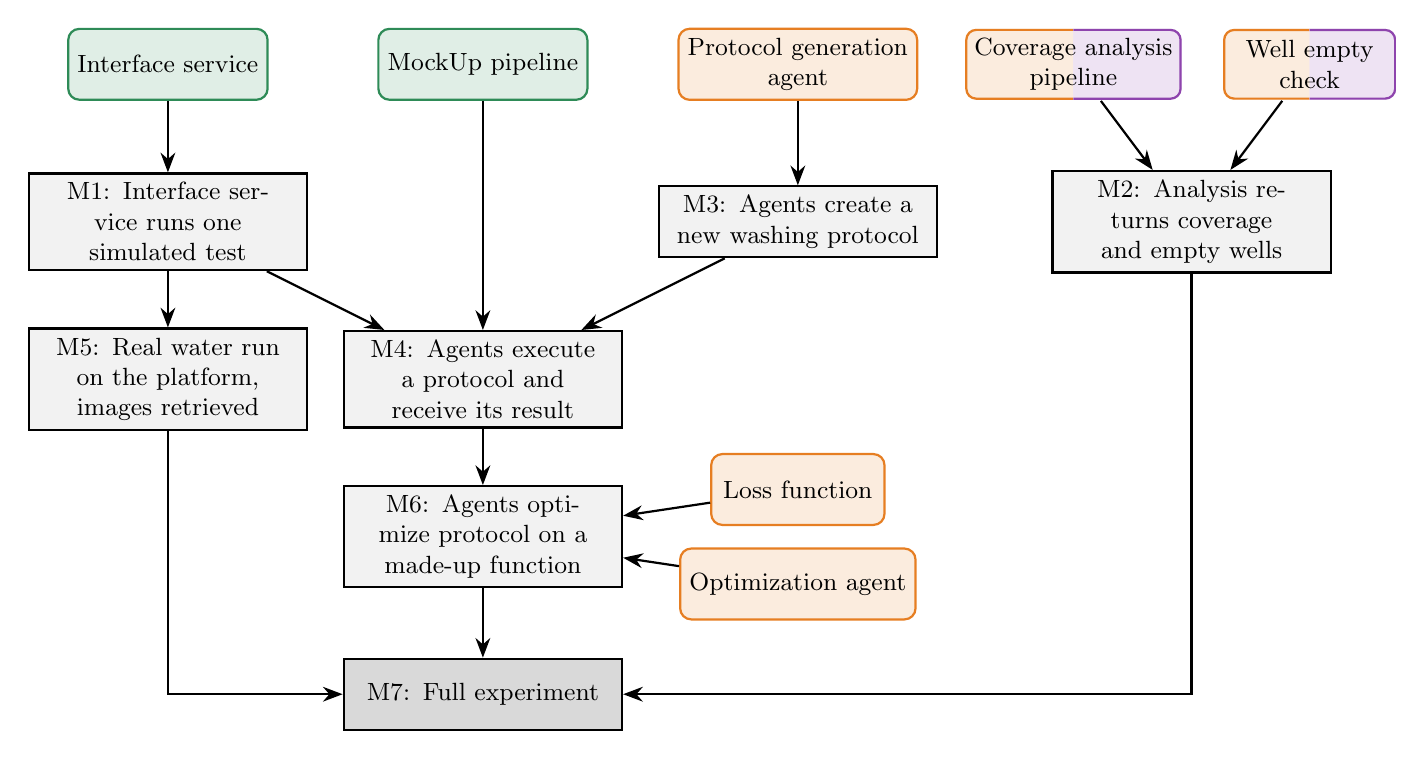
\begin{tikzpicture}[comp/.append style={minimum width=2.2cm}]
    % components
    \node[stefan]  (c_if)    at (0,0)      {Interface service};
    \node[stefan]  (c_mock)  at (4,0)      {MockUp pipeline};
    \node[chris]   (c_gen)   at (8,0)      {Protocol generation\\agent};
    \node[both]    (c_cov)   at (11.5,0)   {Coverage analysis\\pipeline};
    \node[both]    (c_empty) at (14.5,0)   {Well empty\\check};
    \node[chris]   (c_loss)  at (8,-5.4)   {Loss function};
    \node[chris]   (c_opt)   at (8,-6.6)   {Optimization agent};

    % milestones
    \node[milestone] (m1) at (0,-2)    {M1: Interface service runs one simulated test};
    \node[milestone] (m3) at (8,-2)    {M3: Agents create a new washing protocol};
    \node[milestone] (m2) at (13,-2)   {M2: Analysis returns coverage and empty wells};
    \node[milestone] (m4) at (4,-4)    {M4: Agents execute a protocol and receive its result};
    \node[milestone] (m5) at (0,-4)    {M5: Real water run on the platform, images retrieved};
    \node[milestone] (m6) at (4,-6)    {M6: Agents optimize protocol on a made-up function};
    \node[milestone, fill=gray!30] (m7) at (4,-8) {M7: Full experiment};

    \draw[flow] (c_if)    -- (m1);
    \draw[flow] (c_mock)  -- (m4);
    \draw[flow] (c_gen)   -- (m3);
    \draw[flow] (c_cov)   -- (m2);
    \draw[flow] (c_empty) -- (m2);
    \draw[flow] (m1) -- (m4);
    \draw[flow] (m3) -- (m4);
    \draw[flow] (m1) -- (m5);
    \draw[flow] (m4) -- (m6);
    \draw[flow] (c_loss) -- (m6);
    \draw[flow] (c_opt)  -- (m6);
    \draw[flow] (m5) |- (m7);
    \draw[flow] (m6) -- (m7);
    \draw[flow] (m2) |- (m7);
\end{tikzpicture}
\caption{Road map. Coloured boxes are components (by person), grey boxes are milestones.}
\label{fig:roadmap}
\end{figure}

\subsection{Milestones}
\begin{itemize}
    \item Stefan interface service executes one simulated test and provides the results
    \item The image analysis pipeline returns coverage pecentage and whther wells were empty of images
    \item Chis agents create a new washing protocol
    \item Chris agent execute a washing protocol and receive its result from the analysis pipeline
    \item A real single waterrun is executed on the platform and the images retrieved
    \item Chris agents optimize the protocol acording to some made up function
    \item Full experiment
\end{itemize}

\section{Questions}
\begin{itemize}
    \item Can we use multiple squids?
    \item How can the check whether all wells are empty be automized?
    \item Do we need to checkafter every washing step?
    \item Do we only go for 12 washes or create the oracle for any numer of washes?
\end{itemize}

\end{document}
